\documentclass[10pt]{article}
\usepackage[utf8]{inputenc}
\usepackage[T1]{fontenc}
\usepackage{microtype}
\setlength{\emergencystretch}{3em}
\hyphenpenalty=1000
\tolerance=1500
\usepackage[margin=1in,left=1.25in,right=1.25in,top=1in,bottom=1in]{geometry}
\usepackage{algorithm}
\usepackage{algorithmic}
\usepackage[linktoc=all,bookmarksdepth=3,pdfstartview=FitH]{hyperref}
\hypersetup{colorlinks=true,linkcolor=blue,filecolor=magenta,urlcolor=cyan}
\urlstyle{same}
\usepackage{amsmath}
\usepackage{amsfonts}
\usepackage{amssymb}
\usepackage{graphicx}
\usepackage[dvipsnames]{xcolor}
\usepackage{booktabs}
\usepackage{multirow}
\usepackage{amsthm}
\usepackage{enumitem}

\newtheorem{proposition}{Proposition}[section]
\newtheorem{remark}[proposition]{Remark}

\newcommand{\method}{BAPR}
\newcommand{\mode}{z}
\newcommand{\refmode}{r}
\newcommand{\gain}{G}
\newcommand{\clip}{\operatorname{clip}}

\title{BAPR: Belief-Aware Policy Reparameterization for Persistent Actuator Regimes\footnote{Code available at \url{https://github.com/erzhu419/BAPR}}}

\author{
  Yifan Zhang\thanks{Central South University, \href{mailto:erzhu419@gmail.com}{erzhu419@gmail.com}, \href{mailto:204201048@csu.edu.cn}{204201048@csu.edu.cn}} \and
  Liang Zheng\thanks{Central South University, \href{mailto:zhengliang@csu.edu.cn}{zhengliang@csu.edu.cn}}
}
\date{}

\begin{document}
\maketitle

\begin{abstract}
Piecewise-stationary control is often approached by learning a context-conditioned policy or by switching among mode-specific policies. These approaches entangle two problems: identifying the current dynamics and learning a compatible controller. We study a structured but practically relevant alternative in which persistent actuator regimes differ by known, invertible action-coordinate transforms. We introduce \textbf{BAPR} (Belief-Aware Policy Reparameterization), which keeps one canonical policy, infers the current regime from completed transitions, and transforms each canonical action into the current actuator coordinates. A five-head inverse-dynamics ensemble estimates the executed action from $(s_t,s_{t+1})$; a sticky hidden Markov model accumulates causal mode evidence; and the posterior mode determines an exact sign compensation before the next action.

In a prospectively registered HalfCheetah study with ten new policy seeds and new evaluation streams, every learned control arm receives 8.4 million policy-environment interactions. BAPR obtains a switching return of 3297.1, compared with 2287.1 for SAC, 2046.0 for recurrent ESCP, and 2360.2 for RE-SAC. Paired mean improvements are 1009.9 (95\% CI 391.7--1628.2), 1251.1 (553.5--1948.7), and 936.9 (337.1--1536.7), respectively. The causal estimator reaches 98.55\% mode accuracy, has a median switch delay of three steps, and passes oracle-recovery and stationary-retention checks for all ten seeds. The preregistered overall decision nevertheless remains negative: the SAC comparison wins 7/10 policy seeds and 23/30 seed-event cells, below the frozen 8/10 and 24/30 consistency thresholds. The result supports causal action-coordinate compensation for persistent, identifiable actuator-polarity regimes; it does not establish a general solution to arbitrary non-stationarity.
\end{abstract}

\noindent\textbf{Keywords:} non-stationary reinforcement learning; online system identification; action compensation; latent regimes; robust control; Soft Actor-Critic.

\section{Introduction}

Robotic and transportation systems rarely operate under one fixed transition model. Actuators can be recalibrated, channels can fail, traffic can enter a new demand regime, and the active dynamics can remain stable for a period before changing abruptly. This motivates the piecewise-stationary Markov decision process, in which an unobserved regime indexes the transition kernel and changes within an episode~\cite{Padakandla2020Survey,Lecarpentier2019NonStationary}.

Most adaptive reinforcement-learning methods address this setting by conditioning a policy on recent experience or by selecting among separately trained policies~\cite{Luo2022ESCP,Rakelly2019PEARL,Zintgraf2020VariBAD}. This is appropriate when different regimes require genuinely different decision rules. It is unnecessarily difficult, however, when regimes are related by a known coordinate transformation. Independently optimized policies can develop incompatible gaits even when their physical objectives are equivalent. A learned router must then identify the regime and switch between controllers whose internal conventions are not aligned. The resulting discontinuity can be more damaging than the regime change itself.

This paper separates \emph{mode inference} from \emph{control}. We consider persistent actuator regimes whose executed action is a known transform of the commanded action plus small transition noise. One canonical policy is trained in a fixed reference coordinate system. At deployment, an inverse-dynamics model estimates which transform is active from completed transitions, a sticky Bayesian filter accumulates evidence, and the canonical command is reparameterized into the inferred coordinates. The policy itself is never switched or adapted online.

This design emerged from a sequence of controlled failures. A policy bank with a strong causal router performed well on one HalfCheetah protocol, but a post hoc mechanism audit showed that a single reference policy with exact action compensation was both simpler and stronger. We therefore froze the compensation mechanism, trained fresh reference policies, and conducted a new ten-seed prospective study. The study was designed to distinguish three possible explanations: insufficient mode inference, insufficient oracle headroom, and unstable canonical-controller training.

Our contributions are:
\begin{itemize}[leftmargin=*]
    \item \textbf{A structured adaptation mechanism.} We formulate persistent actuator non-stationarity as an action-coordinate problem and derive an exact compensation map for invertible polarity transforms. The method uses one canonical controller rather than a bank of independently optimized policies.
    \item \textbf{Causal online identification.} A transition-only inverse-dynamics ensemble and sticky hidden Markov posterior infer the active transform. The action at time $t$ uses only transitions completed before $t$.
    \item \textbf{A prospective, equal-policy-budget evaluation.} Ten new HalfCheetah policy seeds and disjoint event streams compare BAPR with SAC~\cite{Haarnoja2018SAC}, recurrent ESCP~\cite{Luo2022ESCP}, and RE-SAC~\cite{Zhang2026RESAC}, each trained with 8.4 million policy-environment interactions.
    \item \textbf{An explicit evidence boundary.} BAPR has statistically resolved mean gains over all three comparators, but misses its preregistered SAC consistency threshold by one seed and one event. Ant, Hopper, Walker2d, and bus evidence is reported as transfer or scope evidence rather than pooled into the HalfCheetah claim.
\end{itemize}

\section{Related work}

\subsection{Non-stationary and context-conditioned reinforcement learning}

Non-stationary RL includes continual learning, hidden-parameter MDPs, change-point methods, and meta-RL~\cite{Khetarpal2020ContinualRL,Doshi-Velez2016HiPMDP,Adams2007BOCD,Nagabandi2019MAML}. Context-conditioned methods infer a latent variable from recent experience and feed it to the actor or critic. ESCP learns an environment-sensitive context for sudden changes~\cite{Luo2022ESCP}; PEARL and VariBAD infer task beliefs for meta-RL~\cite{Rakelly2019PEARL,Zintgraf2020VariBAD}. These methods jointly learn representation and control. BAPR instead exploits a known transformation family: the latent variable selects a coordinate map around a single policy.

Bayesian online change detection maintains a posterior over change histories~\cite{Adams2007BOCD}. BAPR does not use the original run-length-based BOCD and lower-confidence-bound machinery from earlier development versions. Its deployment filter is a finite-state sticky hidden Markov model over actuator regimes. This distinction matters because the current claim concerns causal system identification and action reparameterization, not adaptive critic conservatism.

\subsection{Robust and ensemble reinforcement learning}

Robust MDP methods optimize against transition uncertainty sets~\cite{Iyengar2005RobustDP,Wiesemann2013RobustMDP}, while distributionally robust actor-critic methods extend this idea to function approximation~\cite{Zhou2023NaturalActorCritic,Panaganti2024RobustF}. SAC provides the maximum-entropy off-policy baseline~\cite{Haarnoja2018SAC}. RE-SAC separates aleatoric regularization from epistemic ensemble disagreement and was originally developed for stochastic bus control~\cite{Zhang2026RESAC}. Robust training can produce a useful fallback policy, but a single compromise policy may leave performance on the table when persistent modes require conflicting actuator commands. BAPR asks whether structured compensation can recover that mode-specific headroom without learning multiple deployment policies.

\subsection{System identification and policy reparameterization}

Hidden-parameter and contextual RL infer dynamics variables that are not directly observed~\cite{Doshi-Velez2016HiPMDP,Benjamins2021CARL}. Our setting is narrower: the candidate actuator transforms are known, while the active transform is hidden. The inverse model therefore predicts the physical action implied by a transition, and the Bayesian filter compares this prediction with each candidate transformed command. This separation makes the estimator interpretable and provides a true-mode oracle that isolates controller headroom from inference error.

\section{Problem formulation}
\label{sec:problem}

We consider a piecewise-stationary MDP with continuous state $s_t\in\mathcal{S}$ and commanded action $a_t\in[-1,1]^d$. A latent regime $z_t\in\{0,\ldots,M-1\}$ remains fixed for a dwell interval and may change within an episode. The environment applies a regime-dependent action transform before the physics step:
\begin{equation}
    u_t = \clip\!\left(\gain_{z_t} a_t + \varepsilon_t,-1,1\right),
    \label{eq:executed_action}
\end{equation}
where $u_t$ is the executed action, $\gain_z$ is a known diagonal transform, and $\varepsilon_t$ is zero-mean actuator noise. The transition and reward are generated from $(s_t,u_t)$. The agent observes $(s_t,a_t,r_t,s_{t+1})$ but not $u_t$ or $z_t$.

The primary benchmark uses $M=4$ polarity transforms. For HalfCheetah's six action dimensions, the affected channel sets are the lower half, upper half, even indices, and odd indices. Affected channels have gain $-1$ and the remaining channels gain $+1$. Thus each $\gain_z$ is diagonal, orthogonal, and self-inverse: $\gain_z^{-1}=\gain_z$. All modes share the same robot physics and additive actuator-noise standard deviation 0.02. The mode persists for 250 environment steps.

The objective is not to learn an arbitrary universal policy. We seek a controller that (i) preserves the performance of a policy trained in a canonical regime, (ii) infers the active transform causally, and (iii) avoids discontinuities caused by switching among independently optimized policies.

\section{BAPR}
\label{sec:method}

\subsection{Canonical policy and exact action compensation}

Let $r$ denote a fixed reference regime and let $\pi_r(s)$ be a deterministic deployment action from a policy trained in that coordinate system. If the current regime $z$ were known, BAPR would command
\begin{equation}
    a_t^{\mathrm{comp}}
    = \clip\!\left(\gain_z^{-1}\gain_r\pi_r(s_t),-1,1\right).
    \label{eq:compensation_general}
\end{equation}
For polarity transforms, this becomes
\begin{equation}
    a_t^{\mathrm{comp}}
    = \gain_z\gain_r\pi_r(s_t),
    \label{eq:compensation_polarity}
\end{equation}
because sign changes preserve the action bounds.

\begin{proposition}[Pathwise equivalence under arbitrary polarity switching]
\label{prop:equivalence}
Let $(z_t)_{t=0}^{H-1}$ be any regime sequence. Assume that all regimes share the same transition and reward maps and differ only through diagonal sign matrices $\gain_z$. Couple a rollout that remains in reference regime $r$ and a rollout that follows $(z_t)$ by using the same initial simulator state and exogenous-noise sequence. If the latter commands Eq.~\eqref{eq:compensation_polarity} with the true $z_t$ at every step, then the two rollouts have identical executed actions, states, rewards, and finite-horizon return pathwise. Consequently, their return distributions and expectations are equal under the same noise law.
\end{proposition}
\begin{proof}
At equal states, the deterministic canonical policy produces the same reference action. Because $\gain_{z_t}^2=I$, the compensated rollout has
$\gain_{z_t}a_t^{\mathrm{comp}}=\gain_{z_t}\gain_{z_t}\gain_r\pi_r(s_t)=\gain_r\pi_r(s_t)$.
Sign matrices preserve the action box, and adding the coupled noise before the common componentwise clipping therefore gives the same executed action as in regime $r$. The common transition and reward maps give the same next state and reward. Induction over $t$ proves the pathwise claim; equality in distribution follows by taking the same coupling under the common noise law. Appendix~\ref{app:proofs} gives the full construction and assumptions.
\end{proof}

The true-mode controller defined by Eq.~\eqref{eq:compensation_polarity} is a privileged-information reference for the learned estimator and exactly reproduces the reference-regime trajectory under the coupling above. It is not a universal pointwise upper bound on every incorrectly routed action sequence. The uncompensated canonical policy is a necessary lower control: it tests whether the benchmark actually requires the transform.

\subsection{Transition-only inverse system identification}

The executed action is not exposed to the agent. We train an ensemble $\{f_j\}_{j=1}^{K}$ to infer it from the observed transition:
\begin{equation}
    \hat u_t^{(j)} = f_j\!\left(
        \tanh(s_t/5),\tanh(s_{t+1}/5),
        \tanh((s_{t+1}-s_t)/0.1)
    \right).
\end{equation}
The estimator does not receive the commanded action as an input. The command is used only after prediction to score candidate regimes. For candidate mode $z$, the implied executed command is
\begin{equation}
    \tilde u_t(z)=\clip(\gain_z a_t,-1,1).
\end{equation}
With empirical diagonal residual variance $\sigma^2$, the ensemble emission score is
\begin{equation}
    \ell_t(z)=\log\frac{1}{K}\sum_{j=1}^{K}
    \exp\left[-\frac{1}{2d}\sum_{q=1}^{d}
    \left(
      \frac{(\tilde u_{t,q}(z)-\hat u_{t,q}^{(j)})^2}{\sigma_q^2}
      +\log(2\pi\sigma_q^2)
    \right)\right].
    \label{eq:emission}
\end{equation}
The frozen five-head estimator uses three-layer multilayer perceptrons with width 256. It was trained for 1,500 updates on trajectories disjoint from the prospective policy and evaluation seeds. The estimator is a separately pretrained component; its data are not counted as part of the equal 8.4M policy-interaction budget, and this additional supervision is reported as a limitation.

\subsection{Sticky posterior and causal execution}

Let $b_t(z)$ be the mode posterior available before selecting action $a_t$. A sticky transition prior with hazard $h$ is
\begin{equation}
    \bar b_t(z)=(1-h)b_t(z)+\frac{h}{M-1}\left(1-b_t(z)\right).
\end{equation}
After transition $t$ is completed, BAPR updates
\begin{equation}
    b_{t+1}(z)\propto \bar b_t(z)^{\delta}
    \exp\!\left(c\,\ell_t(z)\right),
    \label{eq:posterior}
\end{equation}
with $h=0.002$, evidence scale $c=1$, and posterior decay $\delta=0.98$. The next action uses $\hat z_{t+1}=\arg\max_z b_{t+1}(z)$. This ordering is causal: $a_t$ uses $b_t$, which contains evidence only from transitions before $t$. No true mode ID, current next state, or future transition enters action selection.

\begin{proposition}[Causal deployment]
\label{prop:causality}
Let the information available before action $t$ be
$\mathcal{H}_t=\sigma\!\left(s_0,(a_\tau,r_\tau,s_{\tau+1})_{\tau=0}^{t-1}\right)$.
If $b_0$ is fixed, the inverse model and posterior update are frozen, and $\arg\max$ uses fixed tie-breaking, then $b_t$, $\hat z_t$, and the deployed action $a_t$ in Algorithm~\ref{alg:bapr} are $\mathcal{H}_t$-measurable. In particular, $a_t$ uses neither $s_{t+1}$ nor future transitions or the unobserved true mode label.
\end{proposition}
\begin{proof}
The claim holds at $t=0$ because $b_0$ is fixed. If $b_t$ is $\mathcal{H}_t$-measurable, then $\hat z_t$ and $a_t$ are deterministic functions of $(b_t,s_t)$. After $(r_t,s_{t+1})$ is observed, the frozen inverse model, emission score, and Eq.~\eqref{eq:posterior} make $b_{t+1}$ a deterministic function of $\mathcal{H}_{t+1}$. Induction proves the claim. Appendix~\ref{app:proofs} states the information ordering explicitly.
\end{proof}

\begin{algorithm}[t]
\caption{BAPR deployment with a frozen canonical policy}
\label{alg:bapr}
\begin{algorithmic}[1]
\STATE Initialize $b_0(z)=1/M$ and observe $s_0$
\FOR{$t=0,1,\ldots$}
    \STATE $\hat z_t\leftarrow\arg\max_z b_t(z)$
    \STATE $a_t^{\mathrm{ref}}\leftarrow\pi_r(s_t)$
    \STATE $a_t\leftarrow\gain_{\hat z_t}^{-1}\gain_r a_t^{\mathrm{ref}}$
    \STATE Execute $a_t$ and observe $(r_t,s_{t+1})$
    \STATE Predict $\{\hat u_t^{(j)}\}_{j=1}^{K}$ from $(s_t,s_{t+1})$
    \STATE Compute $\ell_t(z)$ for every mode using Eq.~\eqref{eq:emission}
    \STATE Update $b_{t+1}$ using Eq.~\eqref{eq:posterior}
\ENDFOR
\end{algorithmic}
\end{algorithm}

Figure~\ref{fig:v32_method} summarizes the separation between persistent actuator coordinates, causal mode inference, and action reparameterization.

\begin{figure}[t]
\centering
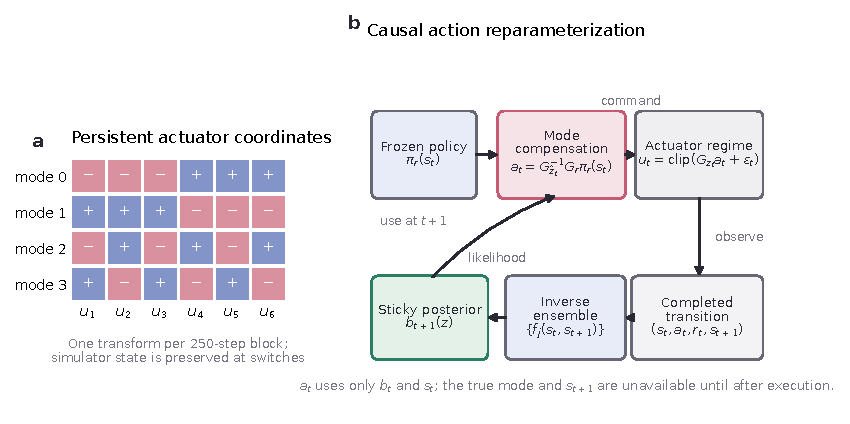
\includegraphics[width=\textwidth]{fig_v32_method.pdf}
\caption{BAPR mechanism for persistent actuator-polarity regimes. \textbf{a}, The four known transforms alter the signs of fixed actuator channels while preserving robot physics, noise scale, and simulator state across 250-step blocks. \textbf{b}, The frozen canonical policy emits an action in reference coordinates. The posterior available before step $t$ selects the inverse transform used for $a_t$. Only after the action is executed does $(s_t,a_t,r_t,s_{t+1})$ update the inverse ensemble and posterior $b_{t+1}$, which can affect the next action but not the current one.}
\label{fig:v32_method}
\end{figure}

\subsection{Controller training}

For each prospective policy seed, the canonical path first trains a SAC source policy for 5.6M interactions over the actuator-regime family and then fine-tunes the complete actor--critic state for 2.8M interactions in fixed reference mode 0. The final policy is used without checkpoint selection. The resulting 8.4M interactions and 525,000 gradient updates match the budgets of SAC, recurrent ESCP, and RE-SAC. BAPR does not update the policy, critic, or estimator during evaluation.

\section{Experiments}
\label{sec:experiments}

\subsection{Questions and protocol}

We ask four questions: (Q1) Does causal compensation improve switching return over equal-budget SAC, ESCP, and RE-SAC? (Q2) Is any gain explained by mode inference rather than access to a stronger controller? (Q3) How consistent is the improvement across independently trained policies and event streams? (Q4) Where does the mechanism cease to apply?

The primary experiment is a prospective HalfCheetah-v2 confirmation registered before training. A five-seed fresh-policy pilot was used only to select a sample size of ten and is not pooled with the confirmation. The confirmation uses ten new policy seeds, three new stationary event streams, and three new switching event streams. Each switching episode lasts 1,000 steps and visits all four modes in 250-step blocks; schedules and starting modes vary by event stream and episode. Stationary evaluation fixes one mode for the full episode. Policies are evaluated deterministically, while actuator noise remains active.

The learned arms are equal in policy-environment interactions: SAC, recurrent ESCP, RE-SAC, and the BAPR canonical path each receive 8.4M interactions and 525,000 updates per policy seed. We additionally report the 5.6M robust source, the uncompensated canonical policy, and true-mode compensation. The primary statistic is the paired switching-return difference across policy seeds. Two-sided 95\% confidence intervals use a paired $t$ interval with nine degrees of freedom.

The preregistered success gate requires, against each equal-budget comparator: (i) a positive paired mean; (ii) a positive lower 95\% confidence bound; (iii) at least 8/10 policy-seed wins; and (iv) at least 24/30 seed-event wins. Mechanism checks additionally require oracle headroom, recovery of at least 70\% of positive oracle gain, and at least 95\% stationary oracle retention for at least eight seeds.

\subsection{Primary confirmation results}

\begin{table}[t]
\centering
\caption{Prospective confirmation returns averaged over ten new HalfCheetah policy seeds. Every learned final control arm has an 8.4M policy-interaction budget. The 5.6M source is diagnostic.}
\label{tab:v32_returns}
\begin{tabular}{lrr}
\toprule
Method & Switching & Stationary \\
\midrule
Robust SAC source, 5.6M & 1650.8 & 1775.0 \\
SAC, 8.4M & 2287.1 & 2382.6 \\
Canonical, no compensation & 340.3 & 560.3 \\
Canonical + true mode & 3422.0 & 3432.5 \\
\textbf{BAPR, causal compensation} & \textbf{3297.1} & \textbf{3403.5} \\
Recurrent ESCP, 8.4M & 2046.0 & 2117.0 \\
RE-SAC, 8.4M & 2360.2 & 2435.9 \\
\bottomrule
\end{tabular}
\end{table}

Table~\ref{tab:v32_returns} shows a large gap between the uncompensated canonical policy and both compensated variants. This establishes that the modes require action reparameterization: a strong mode-0 controller is not a robust controller when its action signs are interpreted in another coordinate system. Causal BAPR recovers most of the true-mode result, reaching 3297.1 switching return and 3403.5 stationary return.

\begin{table}[t]
\centering
\caption{Paired prospective switching comparisons. ``Seeds'' counts positive policy-seed differences; ``events'' counts positive seed--event cells.}
\label{tab:v32_paired}
\begin{tabular}{lrrrrc}
\toprule
Comparison & Difference & 95\% CI & Seeds & Events & Gate \\
\midrule
BAPR $-$ no compensation & $+2956.8$ & $[2500.7,3412.8]$ & 10/10 & 30/30 & pass \\
BAPR $-$ source SAC, 5.6M & $+1646.2$ & $[1174.9,2117.6]$ & 10/10 & 30/30 & pass \\
BAPR $-$ SAC, 8.4M & $+1009.9$ & $[391.7,1628.2]$ & 7/10 & 23/30 & fail \\
BAPR $-$ ESCP, 8.4M & $+1251.1$ & $[553.5,1948.7]$ & 9/10 & 25/30 & pass \\
BAPR $-$ RE-SAC, 8.4M & $+936.9$ & $[337.1,1536.7]$ & 9/10 & 27/30 & pass \\
\bottomrule
\end{tabular}
\end{table}

The paired mean advantage is statistically resolved for every equal-budget comparator (Table~\ref{tab:v32_paired} and Fig.~\ref{fig:v32_results}). Relative to comparator means, BAPR improves switching return by 44.2\% over SAC, 61.1\% over ESCP, and 39.7\% over RE-SAC. The preregistered overall decision is nevertheless \textbf{FAIL}, because the SAC comparison falls one policy seed and one seed--event cell short of the frozen consistency thresholds. We retain this decision rather than replacing it with a post hoc mean-only criterion.

\begin{figure}[t]
\centering
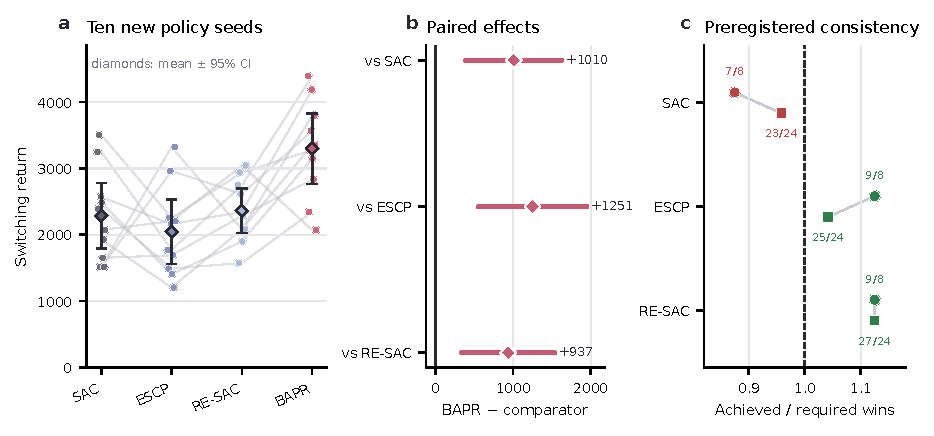
\includegraphics[width=\textwidth]{fig_v32_results.pdf}
\caption{Prospective confirmation results on ten new HalfCheetah policy seeds. \textbf{a}, Switching return for the four equal-budget learned arms. Thin lines connect the same policy-seed index across independently trained methods; diamonds show the mean and two-sided 95\% $t$ interval over $n=10$ policy seeds. \textbf{b}, Paired BAPR-minus-comparator mean differences and 95\% intervals over the same ten seeds. \textbf{c}, Consistency counts relative to the preregistered requirements. Circles denote policy-seed wins out of the required eight and squares denote seed--event wins out of the required 24; the dashed line is the passing threshold. The SAC comparison reaches only 7/8 and 23/24 of the required counts, so the frozen overall decision is negative despite its positive paired interval.}
\label{fig:v32_results}
\end{figure}

\subsection{Mechanism diagnostics}

The causal estimator attains 98.55\% mode accuracy and a median switch-detection delay of three steps. Oracle recovery passes for 10/10 policy seeds, and stationary retention passes for 10/10. Proposition~\ref{prop:equivalence} is also verified numerically in the preceding mechanism audit: with paired simulator states and noise, true-mode compensation has zero maximum executed-signal and return error relative to native reference-mode execution.

The three SAC non-wins occur at policy seeds 88021, 88039, and 88179. Their true-mode oracle headroom over SAC is only $+2.3\%$, $-2.3\%$, and $+4.1\%$, while causal BAPR still recovers 95.4\%, 95.4\%, and 95.5\% of each seed's oracle result. This separates the failure modes. The estimator is not collapsing on these seeds; instead, the trained canonical controller provides little or no advantage over SAC even with privileged mode information. The remaining variance is therefore controller-side rather than inference-side.

\begin{figure}[t]
\centering
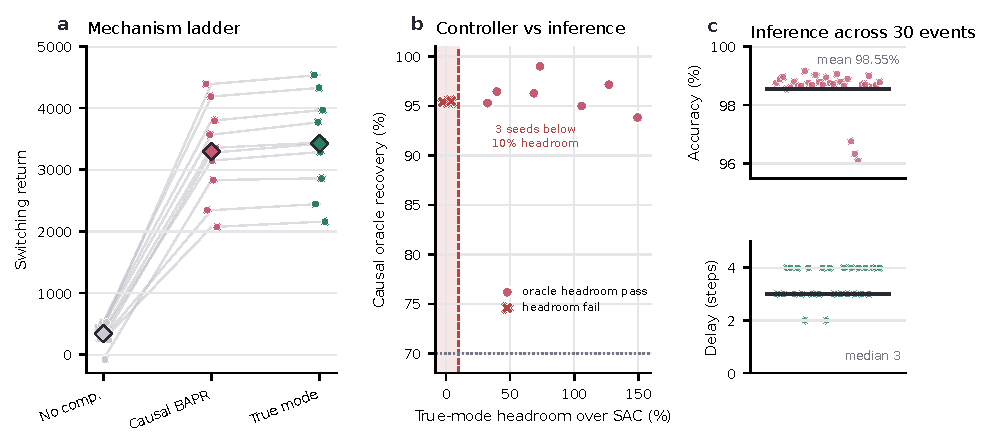
\includegraphics[width=\textwidth]{fig_v32_diagnostics.pdf}
\caption{Mechanism diagnostics separate controller headroom from inference quality. \textbf{a}, Per-seed switching returns for the uncompensated canonical policy, causal BAPR, and true-mode compensation; thin lines connect the same canonical policy and diamonds show means. \textbf{b}, True-mode headroom over equal-budget SAC versus the fraction of the no-compensation-to-oracle gain recovered by causal BAPR. The vertical dashed line marks the registered 10\% headroom requirement and the horizontal dotted line marks 70\% causal recovery. Crosses are the three seeds that lack controller headroom; their causal recovery nevertheless remains above 95\%. \textbf{c}, Event-level inference diagnostics over 30 policy-seed--event cells. Horizontal bars show mean mode accuracy (98.55\%) and median switch-detection delay (3 steps).}
\label{fig:v32_diagnostics}
\end{figure}

\subsection{Developmental and transfer evidence}
\label{sec:scope_evidence}

The prospective ten-seed confirmation is the only result used for the primary statistical claim. Earlier experiments explain why this architecture was selected but are not pooled. A five-seed mechanism audit reused frozen policies and found 4076.2 switching return for causal compensation versus 1424.8 for robust SAC and 3246.0 for a causally routed policy bank. A subsequent fresh-policy pilot trained five new policy seeds; its mean was favorable, but confidence intervals against SAC and RE-SAC crossed zero. The pilot was therefore used only for prospective sample-size planning.

Transfer results define the current scope. A three-seed Ant true-mode audit showed return headroom for compensation (4510.7 versus 2588.6 for robust SAC), but failed its absolute termination-safety gate, so no causal Ant claim is made. Hopper and Walker2d headroom screens terminated before the first scheduled switch in all tested episodes, making those protocols invalid tests of adaptation. The stochastic bus environment remains an important positive domain for RE-SAC-derived robustness~\cite{Zhang2026RESAC,Zhang2026SingleAgentBus}, but it does not expose the known invertible action symmetry required by Eq.~\eqref{eq:compensation_general}; its results are therefore not presented as evidence for the action-compensation mechanism.

\section{Discussion}

\subsection{What the result establishes}

The central empirical finding is not that a generic belief-conditioned policy solves non-stationarity. It is that a persistent actuator-regime problem can become substantially easier after choosing the correct representation. In the tested polarity family, the environment modes are equivalent up to an action-coordinate transform. Learning a policy per mode introduces avoidable controller mismatch; learning one policy and estimating only the transform preserves a common gait. The high causal recovery and short delay show that online identification is sufficiently accurate for this mechanism.

The oracle ladder is essential. Without the no-compensation and true-mode controls, a strong mean return could be attributed either to a better policy seed or to successful mode inference. Here, no compensation fails sharply, true-mode compensation supplies a privileged empirical ceiling for the same canonical policy, and the learned estimator consistently approaches that reference. This ceiling is empirical rather than a mathematical upper bound over arbitrary action sequences. Conversely, the three SAC non-wins reveal that perfect inference cannot create controller headroom that training did not produce.

\subsection{Limitations}

The current evidence has four clear limits. First, the primary confirmation covers one environment and one structured transform family. Known polarity matrices are a stronger assumption than unknown mass, friction, terrain, or morphology changes. Second, the estimator is pretrained on separate specialist trajectories; the comparison equalizes policy interactions, not total end-to-end data collection. Third, the strict preregistered overall gate fails against SAC despite a positive paired confidence interval, so BAPR should be described as having a strong average advantage with controller-seed heterogeneity, not as uniformly superior. Fourth, HalfCheetah has no health-termination constraint. The Ant audit shows that return headroom does not by itself establish safe transfer.

These limits suggest a concrete next step: learn or identify a broader invertible actuator calibration family while retaining the same canonical-controller and oracle-ladder protocol. Extending BAPR to arbitrary dynamics changes would require a different mechanism, not another threshold adjustment to the current posterior.

\section{Conclusion}

We presented BAPR, a belief-aware policy reparameterization method for persistent actuator regimes. BAPR separates causal mode inference from control by combining a frozen canonical policy, a transition-only inverse-dynamics ensemble, a sticky mode posterior, and an exact action-coordinate compensation map. In a prospective ten-seed HalfCheetah study, BAPR has statistically resolved mean gains over equal-budget SAC, recurrent ESCP, and RE-SAC, while recovering the true-mode oracle with high accuracy and short delay. The preregistered overall decision remains negative because consistency against SAC misses the frozen seed and event thresholds. The evidence therefore supports a narrower conclusion: when non-stationarity is an identifiable invertible actuator transformation, policy reparameterization can outperform both robust single policies and learned context adaptation, but controller quality still determines whether adaptation has exploitable headroom.

\section*{Acknowledgments}
The authors thank the developers of JAX, Brax, and the open-source reinforcement-learning ecosystem used in this study.

\clearpage
\appendix

\section{Actuator-regime benchmark}
\label{app:benchmark}

The prospective confirmation benchmark keeps HalfCheetah morphology, gravity, reward, observation space, and episode horizon fixed. Only the actuator-coordinate transform changes. Before each physics step, the environment applies
\begin{equation}
    u_t=\clip(\gain_{z_t}a_t+\varepsilon_t,-1,1),
    \qquad \varepsilon_t\sim\mathcal{N}(0,0.02^2 I).
\end{equation}
For six action dimensions, the four fixed transforms are:
\begin{center}
\begin{tabular}{clc}
\toprule
Mode & Affected channels & $\operatorname{diag}(\gain_z)$ \\
\midrule
0 & lower half & $(-1,-1,-1,+1,+1,+1)$ \\
1 & upper half & $(+1,+1,+1,-1,-1,-1)$ \\
2 & even indices & $(-1,+1,-1,+1,-1,+1)$ \\
3 & odd indices & $(+1,-1,+1,-1,+1,-1)$ \\
\bottomrule
\end{tabular}
\end{center}

The environment holds the active mode fixed for 250 steps. A switching episode contains four blocks and lasts 1,000 steps. The simulator state is preserved at a switch; the robot is not reset. Each mode therefore defines a persistent stochastic transition distribution rather than a per-step resampling of robot morphology.

\section{Proofs for the action-compensation mechanism}
\label{app:proofs}

\subsection{Benchmark assumptions and pathwise equivalence}

The theoretical claim is deliberately limited to the structure implemented by the actuator-polarity benchmark. All modes use common transition and reward maps and differ only in the action transform $\gain_z$. Each $\gain_z$ is a diagonal sign matrix, so $\gain_z^{-1}=\gain_z$ and $\gain_z^2=I$. The canonical deployment policy is deterministic, and its output lies in $[-1,1]^d$. For a pathwise comparison, the reference and switched rollouts use the same initial simulator state and the same realization of actuator noise. Any additional simulator or reset randomness can be included in this common exogenous-noise sequence. These assumptions hold for the prospective HalfCheetah evaluator: the transformed, noisy action is passed to both the physics step and the control-cost term in the reward.

Fix an arbitrary horizon $H$ and mode sequence $(z_t)_{t=0}^{H-1}$. Write the fixed-reference rollout as
\begin{align}
    a_t^{\mathrm{ref}} &= \pi_r(s_t^{\mathrm{ref}}), \\
    u_t^{\mathrm{ref}} &= \clip\!\left(
        \gain_r a_t^{\mathrm{ref}}+\varepsilon_t,-1,1\right),
\end{align}
and the switched, true-mode-compensated rollout as
\begin{align}
    a_t^{\mathrm{comp}} &=
        \gain_{z_t}\gain_r\pi_r(s_t^{\mathrm{comp}}), \\
    u_t^{\mathrm{comp}} &= \clip\!\left(
        \gain_{z_t}a_t^{\mathrm{comp}}+\varepsilon_t,-1,1\right).
\end{align}

\begin{proof}[Detailed proof of Proposition~\ref{prop:equivalence}]
At $t=0$, the states are equal by construction. Suppose
$s_t^{\mathrm{comp}}=s_t^{\mathrm{ref}}$. Deterministic deployment then gives the same canonical output in both rollouts. A sign matrix maps $[-1,1]^d$ onto itself, so the compensated command is admissible without changing its value through command clipping. Using $\gain_{z_t}^2=I$,
\begin{align}
u_t^{\mathrm{comp}}
&=\clip\!\left(
\gain_{z_t}\gain_{z_t}\gain_r
\pi_r(s_t^{\mathrm{comp}})+\varepsilon_t,-1,1\right)\\
&=\clip\!\left(
\gain_r\pi_r(s_t^{\mathrm{ref}})+\varepsilon_t,-1,1\right)
=u_t^{\mathrm{ref}}.
\end{align}
Because the transition and reward maps are common across modes, equal current states, executed actions, and coupled exogenous noise imply equal rewards and equal next states. This closes the induction for every $t<H$, irrespective of when or how often $z_t$ changes. The finite-horizon returns are therefore equal for every coupled sample path. Sampling the coupled noise sequence from its common law gives equality of the return distributions and hence of their expectations.
\end{proof}

The result is an exact structural equivalence, not a performance theorem for the learned mode estimator. In particular, mode-classification accuracy alone does not imply a return-gap bound: errors can occur at dynamically sensitive states and compound through later states. The causal estimator's recovery must therefore remain an empirical quantity.

\subsection{Information ordering and causal execution}

Before selecting action $a_t$, deployment has observed
$\mathcal{H}_t=\sigma\!\left(s_0,(a_\tau,r_\tau,s_{\tau+1})_{\tau=0}^{t-1}\right)$.
The posterior $b_t$ contains emissions only through transition $t-1$. The state $s_{t+1}$ first appears after $a_t$ has been executed and may affect $b_{t+1}$ and $a_{t+1}$, but not $a_t$.

\begin{proof}[Detailed proof of Proposition~\ref{prop:causality}]
The initialization $b_0=1/M$ is deterministic and therefore $\mathcal{H}_0$-measurable. Assume $b_t$ is $\mathcal{H}_t$-measurable. Fixed tie-breaking makes $\hat z_t=\arg\max_z b_t(z)$ a deterministic function of $b_t$, and the frozen policy and known transform make $a_t$ a deterministic function of $(s_t,b_t)$. Thus $a_t$ is $\mathcal{H}_t$-measurable. Once the transition is complete, $(a_t,r_t,s_{t+1})$ belongs to $\mathcal{H}_{t+1}$. The frozen inverse model computes its predictions from $(s_t,s_{t+1})$, the emission score additionally uses the already selected $a_t$, and Eq.~\eqref{eq:posterior} deterministically maps these quantities and $b_t$ to $b_{t+1}$. Hence $b_{t+1}$ is $\mathcal{H}_{t+1}$-measurable, completing the induction.
\end{proof}

This proposition establishes absence of deployment-time look-ahead or true-mode leakage. It does not remove the separately reported supervision used to pretrain the inverse model, nor does it claim that the posterior is calibrated or accurate.

\subsection{Why the legacy contraction theory is excluded}

Earlier BAPR development variants used BOCD, lower-confidence-bound critic penalties, RMDM context losses, and belief-weighted Bellman operators. The final deployment mechanism uses none of these components and performs no online actor, critic, or Bellman update. A contraction theorem for a frozen belief-weighted Bellman operator would therefore describe a different algorithm, even if the theorem were mathematically valid. The present theory is restricted to the two properties used by the implemented mechanism: exact pathwise equivalence under the true transform and causal measurability of learned-transform execution.

\section{Estimator details}
\label{app:estimator}

The frozen inverse model has five independently parameterized heads. Every head is a three-hidden-layer MLP of width 256 with sigmoid linear unit (SiLU) activations and a final $\tanh$. The transition feature is
\begin{equation}
    x_t=\left[
      \tanh(s_t/5),
      \tanh(s_{t+1}/5),
      \tanh((s_{t+1}-s_t)/0.1)
    \right].
\end{equation}
Training uses Adam with learning rate $10^{-4}$, weight decay $10^{-5}$, 1,500 updates, and bootstrap batches of 256 per head. The six empirical inverse-residual variances are
\begin{equation}
 (0.1289,0.1030,0.1174,0.1357,0.1063,0.0967).
\end{equation}
Variance is clipped to $[10^{-4},0.25]$ in the model protocol.

The estimator-training policy seed is 4021 and the validation policy seed is 4049. Training event seeds are 154001 and 154013; validation event seeds are 154101 and 154113. These precede and are disjoint from all pilot and prospective-confirmation policy and evaluation seeds. The prospective protocol does not refit the estimator.

The frozen posterior parameters are hazard $0.002$, evidence scale $1.0$, and posterior decay $0.98$. The posterior used for action $t$ is recorded before incorporating transition $(s_t,a_t,r_t,s_{t+1})$. This convention prevents use of the current next state to choose the current action.

\section{Prospective training and evaluation protocol}
\label{app:v32_protocol}

\subsection{Policy budgets}

The canonical path has two stages. A source SAC controller trains for 1,400 iterations with 4,000 environment steps and 250 gradient updates per iteration, totaling 5.6M interactions and 350,000 updates. Its full actor, critic, target critic, and temperature state is then fine-tuned in fixed mode 0 for 700 iterations, adding 2.8M interactions and 175,000 updates. The final canonical policy therefore receives 8.4M interactions and 525,000 updates. No validation checkpoint is selected; the final policy is evaluated.

SAC, recurrent ESCP, and RE-SAC each receive the same 8.4M interactions and 525,000 updates. This is an equal policy-training budget, not an equal end-to-end data budget, because BAPR also uses the separately pretrained frozen inverse model described in Appendix~\ref{app:estimator}.

\subsection{Seeds and event streams}

The ten prospective-confirmation policy seeds are
\begin{equation}
\begin{split}
\{&88003,88021,88039,88057,88079,\\
  &88103,88121,88139,88157,88179\}.
\end{split}
\end{equation}
Stationary event seeds are 197101, 197117, and 197133. Switching event seeds and their base schedules are:
\begin{center}
\begin{tabular}{cc}
\toprule
Event seed & Base mode schedule \\
\midrule
197201 & $(2,0,3,1)$ \\
197217 & $(1,3,0,2)$ \\
197233 & $(3,2,1,0)$ \\
\bottomrule
\end{tabular}
\end{center}
Each event evaluates five episodes. Episode index cyclically rotates the base schedule so the result is not tied to one starting mode. Stationary evaluation uses five episodes per mode and event seed. All policies use deterministic deployment actions; environment noise remains stochastic.

\subsection{Registered decision rule}

The five-seed fresh-policy pilot failed its registered confirmation rule. It was used only to estimate a sample size of ten for the prospective confirmation; no pilot return is pooled with the confirmation. Before prospective training, the algorithm, reference mode, estimator, policy budgets, seeds, event streams, and decision rule were frozen.

For each comparator, the prospective confirmation requires all of the following:
\begin{enumerate}[leftmargin=*]
    \item positive mean paired switching-return difference;
    \item positive lower bound of a two-sided 95\% paired $t$ interval;
    \item at least 8 of 10 positive policy-seed differences;
    \item at least 24 of 30 positive policy-seed--event differences.
\end{enumerate}
The interval is computed from the ten policy-seed mean differences using the $t_{0.975,9}=2.2622$ critical value. Event wins are consistency diagnostics rather than independent samples in the confidence interval.

The mechanism ladder also checks: (i) true-mode compensation has at least 10\% headroom where required; (ii) causal compensation recovers at least 70\% of positive oracle headroom; and (iii) causal stationary return retains at least 95\% of oracle stationary return. At least eight seeds must pass the latter two checks.

\section{Additional result interpretation}
\label{app:additional_results}

\subsection{Why the registered decision fails}

BAPR's mean switching advantages over SAC, ESCP, and RE-SAC all have positive lower 95\% confidence bounds. ESCP and RE-SAC also pass the frozen consistency counts. The SAC comparison is the only blocker: 7/10 seed wins and 23/30 event wins fall below 8/10 and 24/30.

The three non-winning SAC policy seeds are 88021, 88039, and 88179. Their BAPR-minus-SAC switching differences are $-45.1$, $-228.0$, and $-1.2$. True-mode oracle headroom over SAC is only $+2.3\%$, $-2.3\%$, and $+4.1\%$, respectively. Causal-to-oracle recovery remains approximately 95.4--95.5\%. These paired controls locate the heterogeneity in canonical-controller training rather than mode estimation.

\subsection{Developmental evidence is not pooled}

\begin{table}[h]
\centering
\caption{Role of the developmental and confirmatory experiments. The first three rows are diagnostic and are not pooled with the primary ten-seed result.}
\label{tab:development_history}
\small
\begin{tabular}{@{}p{0.18\textwidth}p{0.14\textwidth}p{0.27\textwidth}p{0.29\textwidth}@{}}
\toprule
Study & Environment & Purpose & Outcome \\
\midrule
Mechanism audit & HalfCheetah & reused-policy mechanism test & compensation passed \\
Transfer audit & Ant & true-mode transfer and safety & headroom found; safety gate failed \\
Fresh-policy pilot & HalfCheetah & five-seed sample-size pilot & confirmation failed \\
Prospective test & HalfCheetah & ten-seed confirmatory test & mean CIs pass; SAC consistency fails \\
\bottomrule
\end{tabular}
\end{table}

In the reused-policy mechanism audit, causal compensation obtained 4076.2 switching return, compared with 4291.8 for true-mode compensation, 3246.0 for a causally routed policy bank, and 1424.8 for robust SAC. Mode accuracy was 98.84\% and median delay was three steps. Because this audit reused policies selected during development, it establishes mechanism plausibility rather than independent confirmation.

In the fresh-policy pilot, causal compensation obtained 3400.6 switching return, compared with 2594.3 for SAC, 1901.8 for ESCP, and 1916.1 for RE-SAC. The five-seed paired confidence intervals against SAC and RE-SAC crossed zero, so the pilot remained a failed confirmation and only informed the prospective sample size.

\section{Cross-environment evidence boundary}
\label{app:cross_environment}

The current paper does not claim a homogeneous four-environment benchmark win.
\begin{itemize}[leftmargin=*]
    \item \textbf{Ant.} A three-seed true-mode action-compensation audit obtained 4510.7 switching return versus 2588.6 for robust SAC, but only one seed passed the absolute zero-termination criterion. This demonstrates privileged headroom, not a safe causal deployment result.
    \item \textbf{Hopper and Walker2d.} In the tested structured-channel screen, every robust and oracle switching episode terminated before the first scheduled switch. The benchmark therefore lacked a valid adaptation window and cannot support a BAPR comparison.
    \item \textbf{Bus control.} The bus domain contains persistent changes in speed and demand distributions with per-step stochastic passenger arrivals and traffic variation. RE-SAC-derived robustness is effective there, but its modes are not known invertible actuator transforms. Bus evidence is relevant motivation for stochastic non-stationarity, not direct evidence for the action-compensation mechanism.
\end{itemize}

\begin{thebibliography}{99}

\bibitem{Adams2007BOCD}
{Adams Ryan P.} and {MacKay David J.C.}, ``Bayesian online changepoint detection,'' \emph{arXiv preprint arXiv:0710.3742}, 2007.

\bibitem{Benjamins2021CARL}
{Benjamins Carolin}, {Eimer Theresa}, {Schubert Frederik}, {Biedenkapp Andr\'e}, {Rosenhahn Bodo}, {Hutter Frank}, and {Lindauer Marius}, ``CARL: A benchmark for contextual and adaptive reinforcement learning,'' \emph{NeurIPS Workshop on Ecological Theory of RL}, 2021.

\bibitem{Doshi-Velez2016HiPMDP}
{Doshi-Velez Finale} and {Konidaris George}, ``Hidden parameter Markov decision processes: A semiparametric regression approach for discovering latent task parametrizations,'' in \emph{Proc. Int. Joint Conf. Artificial Intelligence (IJCAI)}, 2016, pp. 1432--1440.

\bibitem{Haarnoja2018SAC}
{Haarnoja Tuomas}, {Zhou Aurick}, {Abbeel Pieter}, and {Levine Sergey}, ``Soft actor-critic: Off-policy maximum entropy deep reinforcement learning with a stochastic actor,'' in \emph{Proc. Int. Conf. Machine Learning (ICML)}, 2018, pp. 1856--1865.

\bibitem{Iyengar2005RobustDP}
{Iyengar Garud N.}, ``Robust dynamic programming,'' \emph{Mathematics of Operations Research}, vol.~30, no.~2, pp. 257--280, 2005.

\bibitem{Khetarpal2020ContinualRL}
{Khetarpal Khimya}, {Riemer Matthew}, {Rish Irina}, and {Precup Doina}, ``Towards continual reinforcement learning: A review and perspectives,'' \emph{Journal of Artificial Intelligence Research}, vol.~75, pp. 1401--1476, 2022.

\bibitem{Lecarpentier2019NonStationary}
{Lecarpentier Erwan} and {Rachelson Emmanuel}, ``Non-stationary Markov decision processes: A worst-case approach using model-based reinforcement learning,'' in \emph{Advances in Neural Information Processing Systems (NeurIPS)}, vol.~32, 2019, pp. 7214--7223.

\bibitem{Luo2022ESCP}
{Luo Fan-Ming}, {Jiang Shengyi}, {Yu Yang}, {Zhang Zongzhang}, and {Zhang Yi-Feng}, ``Adapt to environment sudden changes by learning a context sensitive policy,'' in \emph{Proc. AAAI Conf. Artificial Intelligence}, 2022, pp. 7637--7646.

\bibitem{Nagabandi2019MAML}
{Nagabandi Anusha}, {Clavera Ignasi}, {Liu Simin}, {Fearing Ronald S.}, {Abbeel Pieter}, {Levine Sergey}, and {Finn Chelsea}, ``Learning to adapt in dynamic, real-world environments through meta-reinforcement learning,'' in \emph{Proc. Int. Conf. Learning Representations (ICLR)}, 2019.

\bibitem{Padakandla2020Survey}
{Padakandla Sindhu}, ``A survey of reinforcement learning algorithms for dynamically varying environments,'' \emph{ACM Computing Surveys}, vol.~54, no.~6, pp. 1--25, 2021.

\bibitem{Panaganti2024RobustF}
{Panaganti Kishan}, {Wierman Adam}, and {Mazumdar Eric}, ``Model-free robust $\phi$-divergence reinforcement learning using both offline and online data,'' in \emph{Proc. Int. Conf. Machine Learning (ICML)}, 2024.

\bibitem{Rakelly2019PEARL}
{Rakelly Kate}, {Zhou Aurick}, {Finn Chelsea}, {Levine Sergey}, and {Quillen Deirdre}, ``Efficient off-policy meta-reinforcement learning via probabilistic context variables,'' in \emph{Proc. Int. Conf. Machine Learning (ICML)}, 2019, pp. 5331--5340.

\bibitem{Wiesemann2013RobustMDP}
{Wiesemann Wolfram}, {Kuhn Daniel}, and {Rustem Ber\c c}, ``Robust Markov decision processes,'' \emph{Mathematics of Operations Research}, vol.~38, no.~1, pp. 153--183, 2013.

\bibitem{Zhang2026RESAC}
{Zhang Yifan} and {Zheng Liang}, ``RE-SAC: Disentangling aleatoric and epistemic risks in bus fleet control: A stable and robust ensemble DRL approach,'' \emph{arXiv preprint arXiv:2603.18396}, 2026.

\bibitem{Zhang2026SingleAgentBus}
{Zhang Yifan}, ``Single Agent Robust Deep Reinforcement Learning for Bus Fleet Control,'' \emph{Transportation Safety and Environment}, tdag005, 2026, doi:10.1093/tse/tdag005.

\bibitem{Zhou2023NaturalActorCritic}
{Zhou Ruida}, {Liu Tao}, {Cheng Min}, {Kalathil Dileep}, {Kumar P. R.}, and {Tian Chao}, ``Natural actor-critic for robust reinforcement learning with function approximation,'' in \emph{Advances in Neural Information Processing Systems (NeurIPS)}, vol.~36, 2023.

\bibitem{Zintgraf2020VariBAD}
{Zintgraf Luisa}, {Shiarlis Kyriacos}, {Igl Maximilian}, {Schulze Sebastian}, {Gal Yarin}, {Hofmann Katja}, and {Whiteson Shimon}, ``VariBAD: A very good method for Bayes-adaptive deep RL via meta-learning,'' in \emph{Proc. Int. Conf. Learning Representations (ICLR)}, 2020.

\end{thebibliography}


\end{document}
